% !TeX root = ../../../book.tex

\subsection{关于像的证明}

你可能已经通过研究我们之前看到的一些例子发现了以下事实。无论如何,我们都可以通过使用像的定义来陈述和证明这个命题。请注意,这是关于\emph{任意}函数的命题;无论 $f$ 是什么,它都成立!

\begin{proposition}\label{prop:proposition7.3.6}
    设 $A,B$ 为集合,$f:A \to B$ 为函数。设 $S, T \subseteq A$,则
    \[Im_f (S \cap T) \subseteq Im_f (S) \cap Im_f (T)\]
\end{proposition}

\begin{proof}
    设 $z \in Im_f (S \cap T)$ 为任意固定元素。这意味着 $\exists a \in S \cap T$ 使得 $f(a) = z$。给定这样的 $a$。

    因为 $a \in S \cap T$,所以我们知道 $a \in S$ 且 $a \in T$。

    因此,根据像的定义,$z \in Im_f (S)$ 且 $z \in Im_f (T)$。

    根据交集的定义,我们推导出 $z \in Im_f (S) \cap Im_f (T)$。

    这证明了我们要证明的集合包含关系。
\end{proof}

为什么我们没有在这里声明\emph{相等}呢?实际上,相等\emph{不一定成立}!也就是说,存在至少一个函数使得逆包含关系 --- 即 $Im_f (S) \cap Im_f (T) \subseteq Im_f (S \cap T)$ --- 不成立。我们将在下面提供这样一个函数的例子。

(你应该尝试想出一个逆包含关系\emph{成立}的函数的例子。这样,我们就能证明不能\emph{必然}得出这个包含关系成立的结论!)

我们将通过示意图来展示一个具有特定属性的例子。然后,我们会使用这个例子来正式\emph{定义}一个函数,并说明其属性,指出这些属性如何与我们的论点相一致。

需要注意的是,使用这种方法是完全可行的,只要你之后补充一个正式的定义。仅仅依靠示意图作为``证明''是不够严谨的,但它确实能帮助你更好地构思证明的\emph{思路}。

另外,在这种情况下,没有必要构造\emph{复杂}或\emph{有趣}的反例。如果你想\emph{反驳}一个全称量化陈述,只需要\emph{一个}有效的例子就可以了!特别是,不要觉得你需要定义一个通过\emph{公式}处理\emph{数字}的函数。有时,这反而会增加难度!通常,反例可以通过只包含几个(如两个或三个)元素的集合来构造。\\

\begin{example}
    我们声称存在集合 $A,B,S,T$ 和函数 $f : A \to B$,使得 $Im_f (S) \cap Im_f (T) \nsubseteq Im_f (S \cap T)$。让我们看看如何构造这样的例子。基于前面的讨论,我们将尝试构造一个包含大约三个元素的集合的例子。我们先令 $A = \{1, 2, 3\}$ 并定义 $f(1)$:

    \begin{center}
        {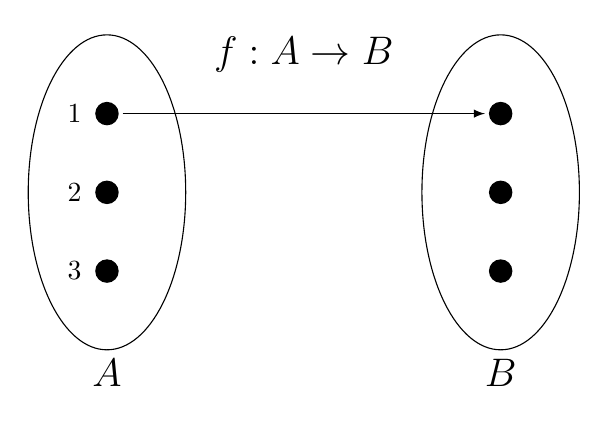
\begin{tikzpicture}[scale=1]
            \foreach \x in  {1,2,3}
            {
                \node at (5, -\x)[circle,fill,inner sep=3pt]{};
            }
            \draw[shift={(5.2, -1)}] node[right] {$\bigstar$};
            \draw (5,-2) ellipse (1 and 2);
    
            \foreach \x in  {1,2,3}
            {
                \node at (0, -\x)[circle,fill,inner sep=3pt]{};
                \draw[shift={(-0.2, -\x)}] node[left] {$\x$};
            }
            \draw (0,-2) ellipse (1 and 2);
    
            \draw[-latex] (0.2,-1) -- (4.8,-1); 
            
            \node[below] at (0, -4){\Large $A$};
            \node[below] at (5, -4){\Large $B$};
            \node[above] at (2.5, -0.6){\Large $f:A \to B$};
        \end{tikzpicture}}
    \end{center}

    为了便于定义,我们令 $S = \{1, 2\}$。让 $S$ 中包含两个元素似乎更合理,因此我们做出这个选择。此外,我们应该设 $f(1) \ne f(2)$,否则 $Im_f(S)$ 只会包含一个元素,这样 $S$ 有两个元素就没有意义了。因此,我们定义 $f(2)$:

    \begin{center}
        {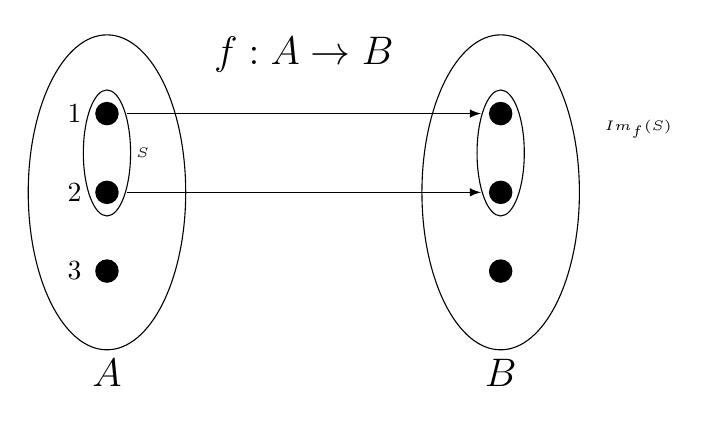
\begin{tikzpicture}[scale=1]
            \foreach \x in  {1,2,3}
            {
                \node at (5, -\x)[circle,fill,inner sep=3pt]{};
            }
            \draw[shift={(5.2, -1)}] node[right] {$\bigstar$};
            \draw[shift={(5.2, -2)}] node[right] {$\square$};
            \draw (5,-2) ellipse (1 and 2);
            \draw (5,-1.5) ellipse (0.3 and 0.8);
    
            \foreach \x in  {1,2,3}
            {
                \node at (0, -\x)[circle,fill,inner sep=3pt]{};
                \draw[shift={(-0.2, -\x)}] node[left] {$\x$};
            }
            \draw (0,-2) ellipse (1 and 2);
            \draw (0,-1.5) ellipse (0.3 and 0.8);
    
            \draw[-latex] (0.25,-1) -- (4.75,-1);
            \draw[-latex] (0.25,-2) -- (4.75,-2); 
    
            \node[right] at (0.25, -1.5){\tiny $S$};
            \node[right] at (6.2, -1.2){\tiny $Im_f(S)$};
            \node[below] at (0, -4){\Large $A$};
            \node[below] at (5, -4){\Large $B$};
            \node[above] at (2.5, -0.6){\Large $f:A \to B$};
        \end{tikzpicture}}
    \end{center}

    现在,我们需要选择集合 $T$。如果让 $S$ 和 $T$ 互不相交 ($S \cap T = \varnothing$) 会很有趣,而如果让 $T$ 包含 $S$ ($T \supseteq S$),处理起来可能会很复杂。因此,我们设 $T = \{2, 3\}$。接下来,我们只需要定义 $f(3)$。在考虑每种情况时,请参照上面的示意图,想象画一个箭头来表示 $f(3)$。

    \begin{itemize}
        \item 如果 $f(3) = f(2) = \square$。\\
            这种情况下,$Im_f(T) = \{\square\}$,所以 $Im_f (S) \cap Im_f (T) = \{\square\}$。而 $Im_f (S \cap T) = \{\square\}$, 这行不通。
        \item 如果 $f(3)$ 等于其他值,比如 $\smiley{}$。\\
            这也行不通。我们会得到 $Im_f (S) \cap Im_f (T) = \{\square\} = Im_f (S \cap T)$。
        \item 如果 $f(3) = f(1) = \bigstar$。\\
            这似乎可以!
    \end{itemize}

    \begin{center}
        {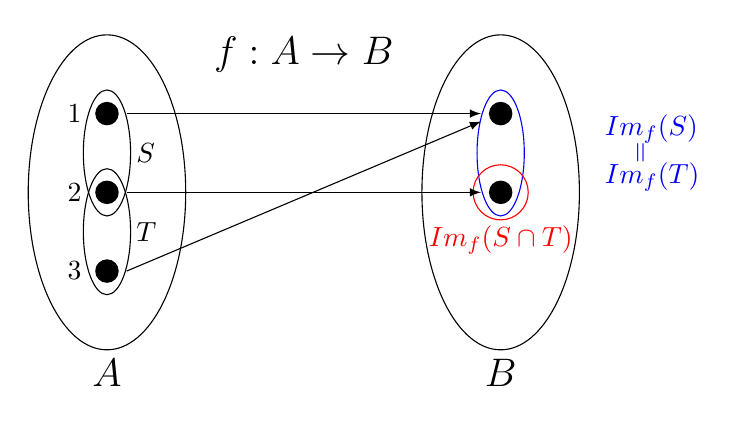
\begin{tikzpicture}[scale=1]
            \foreach \x in {1,2}
            {
                \node at (5, -\x)[circle,fill,inner sep=3pt]{};
            }
            \draw[shift={(5.2, -1)}] node[right] {$\bigstar$};
            \draw[shift={(5.2, -2)}] node[right] {$\square$};
            \draw (5,-2) ellipse (1 and 2);
            \draw[blue] (5,-1.5) ellipse (0.3 and 0.8);
            \draw[red] (5,-2) circle (0.35);
            \node[below, red] at (5, -2.3){$Im_f(S \cap T)$};
    
            \foreach \x in  {1,2,3}
            {
                \node at (0, -\x)[circle,fill,inner sep=3pt]{};
                \draw[shift={(-0.2, -\x)}] node[left] {$\x$};
            }
            \draw (0,-2) ellipse (1 and 2);
            \draw (0,-1.5) ellipse (0.3 and 0.8);
            \draw (0,-2.5) ellipse (0.3 and 0.8);
    
            \draw[-latex] (0.25,-1) -- (4.75,-1);
            \draw[-latex] (0.25,-2) -- (4.75,-2); 
            \draw[-latex] (0.25,-3) -- (4.75,-1.1); 
    
            \node[right] at (0.25, -1.5){$S$};
            \node[right] at (0.25, -2.5){$T$};
            \node[right, blue] at (6.2, -1.2){$Im_f(S)$};
            \node[right, blue, anchor=center, rotate=90] at (6.8, -1.5){$=$};
            \node[right, blue] at (6.2, -1.8){$Im_f(T)$};
            \node[below] at (0, -4){\Large$A$};
            \node[below] at (5, -4){\Large$B$};
            \node[above] at (2.5, -0.6){\Large $f:A \to B$};
        \end{tikzpicture}}
    \end{center}
\end{example}

我们已经成功实现 $Im_f (S) \cap Im_f (T)$ 是 $Im_f (S \cap T)$ 的\emph{真}超集。

回顾一下我们的构造过程,看看你是否理解我们的思路。我们需要遵守哪些限制?在哪些方面有选择的自由?我们最终决定怎么做?

需要说明的是,这绝对不是\emph{唯一的}例子!你也可以尝试想出其他的例子!

现在,我们只需要用我们构造的最终示意图来定义一个例子,并证明它的有效性。我们开始吧!

\begin{proof}
    定义 $A = \{1, 2, 3\}, B = \{\bigstar, \square\}$。

    定义 $f : A \to B$ 为 $f(1) = \bigstar, f(2) = \square, f(3) = \bigstar$。

    定义 $S = \{1, 2\}, T = \{2, 3\}$。

    易得 $S \cap T = \{2\}$,所以 $Im_f (S \cap T) = \{f(2)\} = \{\square\}$。

    然而,$Im_f (S) = Imf (T) = B$,所以 $Im_f (S) \cap Im_f (T) = \{\bigstar, \square\} \ne \{\square\}$。

    因为 $\bigstar \in Im_f (S) \cap Im_f (T)$ 而 $\bigstar \notin Im_f (S \cap T)$,这证明了我们的声明。
\end{proof}

我们已经展示了如何\textbf{证明}关于任意函数和像的声明,以及如何通过\textbf{构造}具体反例来\textbf{反驳}一个声明。在下面的练习中,你将会遇到类似的问题。有时,你需要判断一个声明是否为真。(在这里,我们已经提前告诉你哪个声明是正确的。)我们建议你可以尝试以下两种方法:
\begin{enumerate}[label=(\arabic*)]
    \item 试着证明这个声明,看看是否在某个地方会出现问题;
    \item 试着构造一个反例,看看是否会遇到困难。
\end{enumerate}
如果你完成了上面任意一项……太好了,你已经解决了这个问题!但如果你感到困难,这可能会帮助你更好地理解问题的本质。

具体来说,我们要求你用 ``$\cup$'' 代替 ``$\cap$'' 来重新审视我们上面讨论的命题。你认为会有什么不同吗?试试看吧!